% 函数的连续性
% 极限|微积分|连续函数|左连续|右连续

\pentry{极限\upref{Lim}}

简单来说, \textbf{连续函数}定义为: 在某个区间内, 函数曲线是连续的. 例如常见的 $\sin x$, $\exp x$, $x^2$ 都在整个实数域上连续, 又例如 $\ln x$ 和 $1/x$ 在区间 $(0, \infty)$ 上连续, $\tan x$ 在所有 $x_n = (1/2 + n)\pi$($n$ 为自然数)处不连续, $1/x$ 在 $x = 0$ 处不连续. 但这只是一些简单的情况. 在一些情况下这种判断方法则显得不严谨, 例如 $\sin(1/x)$ 在原点处的连续性(不连续)根据这个定义不好判断. 所以我们需要一个更严谨的定义.

首先我们要讨论函数在一个点附近是否是连续的.这个概念的思想核心是,在函数曲线的某一点附近$(x_0, f(x_0))$,无论我们要求$f(x)$有多接近$f(x_0)$,只要$x$足够靠近$x_0$,就一定能满足条件.比如说,如果定义函数$f$为当$x<0$的时候,$f(x)=0$,其它时候$f(x)=1$,那么在$x=0$这一点处$f$就是跳跃的.如果我们要求的接近程度小于$1$,那么无论$x$多接近$0$,只要$x<0$,$f(x)$和$f(0)=1$的距离就永远满足不了需要.

准确地描述以上“连续”的概念,如下所示:

\begin{definition}{函数在一点的连续性}
函数 $f(x)$ 在某点 $x = x_0$ 处\textbf{连续}的定义是: 函数$f(x)$在某点$x=x_0$处连续,当且仅当对于任何精度要求$\epsilon>0$,我们都可以找到一个对应的范围$\delta>0$,使得只要$|x-x_0|<\delta$,就有$|f(x)-f(x_0)|<\epsilon$.如果一个函数在某区间的所有点都连续, 我们就说它\textbf{在这个区间连续}.

另一个等价说法是常见的:
\begin{equation}
\lim_{x \to x_0} f(x) = f(x_0)
\end{equation}
\end{definition}

注意这里要求 $x$ 从左边和右边趋近于 $x_0$ 时的极限(即左极限和右极限)都成立. % 未完成: 极限词条中介绍左极限和右极限

以上所定义的连续性是针对一个个点$x_0$而言的,就算函数在每一个点都连续,我们也只能说这个函数是\textbf{逐点连续的(pointwise continuous)}.事实上,还有一种更强的连续性,它着眼于整体的性质,这就是\textbf{一致连续(uniformly continuous)}.它的准确定义如下:

\begin{definition}{一致连续}
如果函数$f(x)$在区间$S$上,对于任意精度$\epsilon>0$,都存在对应的范围$\delta>0$,使得只要$|x_1-x_2|<\delta$,那么$|f(x_1)-f(x_2)|<\epsilon$.

\end{definition}

一致连续着眼于整个区间的性质,而不是一个个点.显然,一致连续的函数肯定逐点连续,但是逐点连续的函数不一定一致连续.比如说,考虑函数$f(x)=1/x$,那么在区间$(0, 1)$上,$f$就是逐点连续的,但它并不一致连续;对于同样的精度要求$\epsilon>0$和任何范围$\delta>0$,只要$0<x_1<\delta$,那么就总有一个足够小的$x_2$使得$|f(x_1)-f(x_2)|>\epsilon$,毕竟当$x_2$接近$0$的过程中,$f(x_2)$会越来越趋近于无穷大.

\begin{exercise}{连续但不一致连续的函数}
试证明 $1/x$ 在区间 $(0, +\infty]$ 以及 $x^2$ 在 $\mathbb R$ 都是连续的, 但不是一致连续的.
\end{exercise}

\begin{theorem}{}\label{contin_the1}
设$S$是$\mathbb{R}$的一个区间.函数$f$在$S$上逐点连续的充分必要条件是,对于任何开区间$A\subset \mathbb{R}$,满足$f(x)\in A$的所有$x$构成的集合,是若干开区间的并集.用紧凑的写法来表达就是,$f^{-1}(A)$是开区间的并集.
\end{theorem}

这个定理还可以等价地用闭区间来表达:$f$在$S$上逐点连续的充分必要条件是,任何闭区间的逆映射是闭区间的并集.

\begin{figure}[ht]
\centering
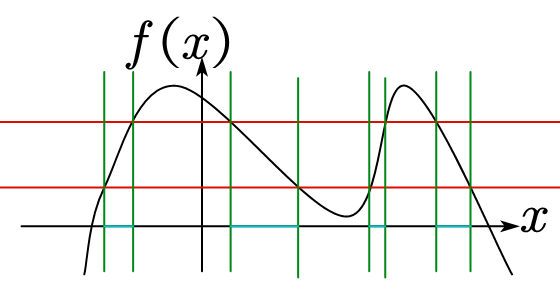
\includegraphics[width=5cm]{./figures/contin_1.png}
\caption{如图,红色水平线在$f(X)$轴上划分出了一个开/闭区间,绿色垂直线是取反函数的过程,$x$轴上的靛蓝色线段就是取反函数的结果.从这个图可以直观地看出\autoref{contin_the1}的意义.} \label{contin_fig1}
\end{figure}

在实数轴上,开集被定义为任何开区间的并集,而闭集是开集的补集.如果$S$是$\mathbb{R}$的一个子集,那么$S$上的开集被定义为$\mathbb{R}$的开集和$S$的交集.这样一来,\autoref{contin_the1}就可以扩展为:$f$在$S$上逐点连续,等价于对于任何开集$A$,$f^{-1}(A)\cap S$是$S$上的开集,等价于对于任何闭集$B$,$f^{-1}(B)\cap S$是$S$上的闭集.

用逆映射来刻画连续性是一个非常好用的方法.
